\newpage
\chapter{Chapter}
\section{Section}
\subsection{Subsection}
\subsubsection{Subsubsection}
My text here with \textbf{italics}, with \textbf{bold}, and a \href{https://davibarreira.github.io/}{link}.  Adding some math expression here with $x=10$ and $x=10$Adding some math expression here with $x=10$ and \begin{displaymath}
	d(\omega(t_0),\omega(t_1)) \leq \int^{t_1}_{t_0}g(s) ds.
\end{displaymath} Adding some code like  \lstinline{plots}. Note that the  \lstinline{using plots} """
\begin{lstlisting}[language=JuliaLocal, style=julia]
using PlutoUI
\end{lstlisting}

\begin{lstlisting}[language=JuliaLocal, style=julia]
begin
	using Plots
	y(x) = sin(x)
	plot(y,
		color=:blue)
end
\end{lstlisting}

\begin{figure}[H]
	\centering
	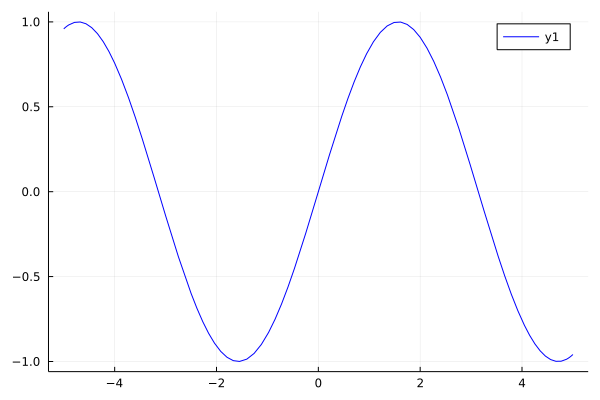
\includegraphics[width=0.8\textwidth]{./figures/notebooktest_figure1.png}
	\label{fig:notebooktest_figure1.png}

\end{figure}

\begin{lstlisting}[language=JuliaLocal, style=julia]
A = [10,10,10]
\end{lstlisting}

\begin{verbatim}
3-element Vector{Int64}:
 10
 10
 10
\end{verbatim}

\begin{lstlisting}[language=JuliaLocal, style=julia]
x = rand(10);
\end{lstlisting}

\begin{lstlisting}[language=JuliaLocal, style=julia]
x .+ 1
\end{lstlisting}

\begin{verbatim}
10-element Vector{Float64}:
 1.0258088405853951
 1.0858707778915404
 1.0714128846249746
 1.67569299652866
 1.1029227939140434
 1.0630875428395277
 1.9438492956457545
 1.6158447871122887
 1.9809914612322974
 1.6483084921096993
\end{verbatim}

\begin{lstlisting}[language=JuliaLocal, style=julia]
set_theme!(theme_ggplot2())
\end{lstlisting}

\begin{lstlisting}[language=JuliaLocal, style=julia]
Makie.plot(x)
\end{lstlisting}

\begin{figure}[H]
	\centering
	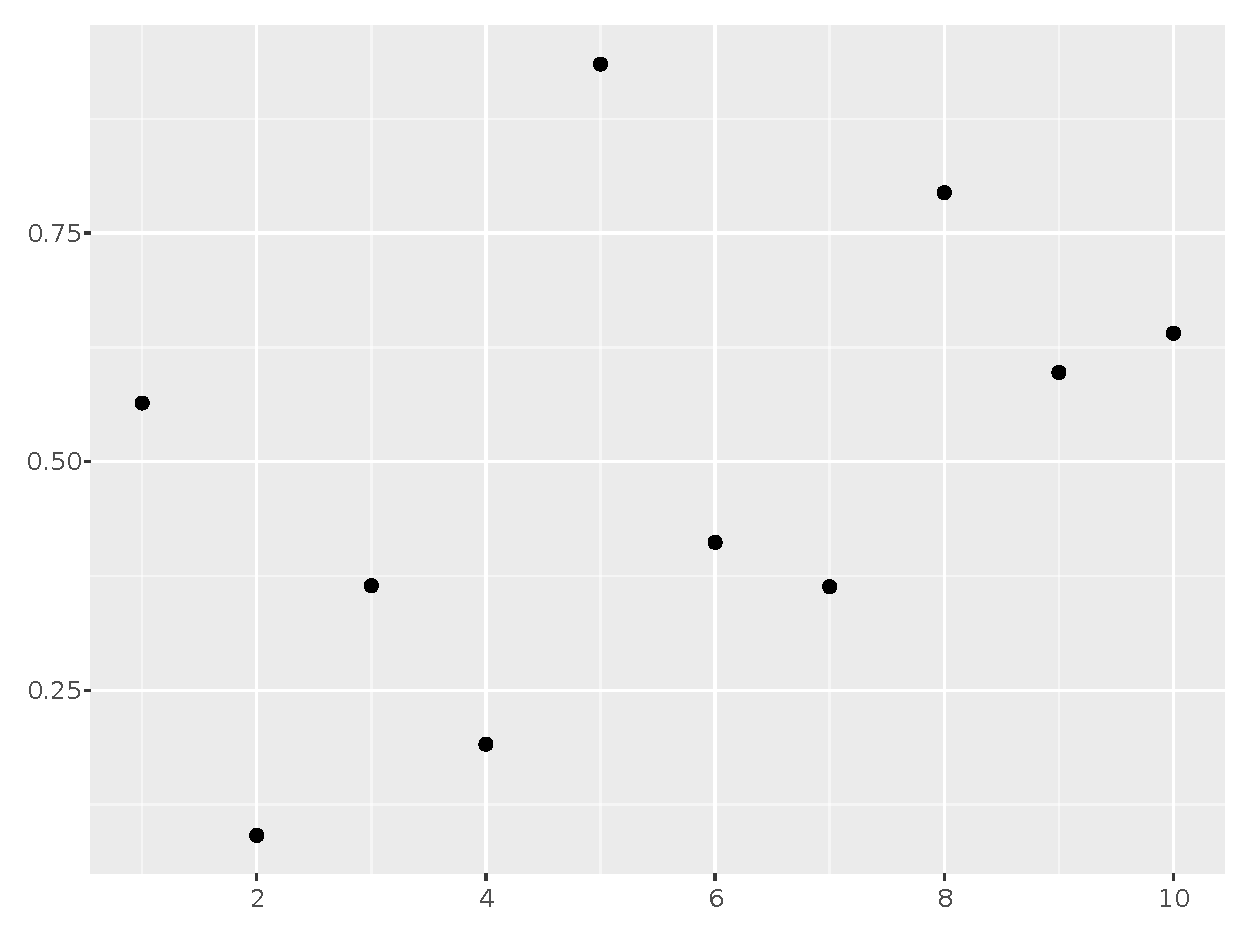
\includegraphics[width=0.8\textwidth]{./figures/notebooktest_figure2.pdf}
	\label{fig:notebooktest_figure2.pdf}

\end{figure}

\begin{lstlisting}[language=JuliaLocal, style=julia]
PlutoUI.LocalResource("figure.svg")
\end{lstlisting}


\begin{lstlisting}[language=JuliaLocal, style=julia]
PlutoUI.LocalResource(figurepath)
\end{lstlisting}

\begin{figure}[H]
	\centering
	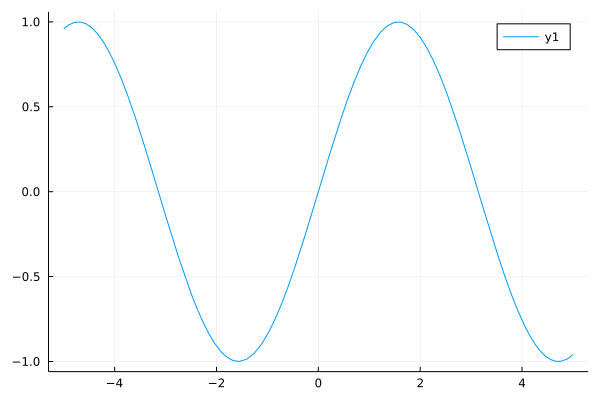
\includegraphics[width=0.8\textwidth]{/home/davibarreira/MEGA/EMAp/NotebookToLatex.jl/test/plotexample.png}
	\label{fig:/home/davibarreira/MEGA/EMAp/NotebookToLatex.jl/test/plotexample.png}

\end{figure}
